\documentclass[a4paper, 12pt]{article}
\usepackage[a4paper,top=1.5cm, bottom=1.5cm, left=1cm, right=1cm]{geometry}
\usepackage[utf8]{inputenc}
\usepackage{mathtext}
\usepackage{amsmath}
\usepackage{amsfonts}
\usepackage[english, russian]{babel}
\usepackage{indentfirst}
\usepackage{longtable}
\usepackage{graphicx}
\graphicspath{{pictures/}}
\DeclareGraphicsExtensions{.pdf,.png,.jpg}
\usepackage{natbib}

\title{Лабораторная работа 1.1.3 Статистическая обработка результатов многократных измерений}
\author{Михаил Колтаков}
\date{7 сентября 2020 г.}


\begin{document}
	\maketitle
	\section*{Цель работы:}
		Применение методов обработки экспериментальных данных при измерении сопротивлений
	\section*{В работе используются:}
		Набор резисторов(270 штук), универсальный цифровой вольтметр, работающий в режиме "Измерение сопротивлений постоянному току"
	\section*{Теория к работе:}
		\subsection*{Обоснование пренебрежения погрешностью омметра}
			Поскольку наш цифровой вольтметр обеспечивает точность до сотых долей процента относительной погрешности, погрешностью измерений, связанных с ним можно пренебречь по сравнению с отклонениями от номинала, полученными в процессе изготовления резисторов.
		\subsection*{Теория статистики}
			Посчитаем среднее сопротивление резисторов
			$$\langle R\rangle = \frac{1}{N} \sum_{i = 1}^{N} R_i - среднее \: значение \: сопротивления \: резистора$$
			N - число резисторов \newline
			$R_i - значение\:сопротивления\:i-того\:резистора$
			\par
			Чтобы охарактеризовать случайные погрешности при изготовлении набора резисторов, необходимо построить гистограмму. Для этого выберем из результатов $R_{макс}$ и $R_{мин}$ и посчитаем интервал изменения сопротивления, разделив разность максимального и минимального значения на m=20 частей.
			$$ \Delta R = \frac{R_{макс}-R_{мин}}{m}$$
			\par
			Гистограмму будем строить следующим образом. По оси абсцисс откладываем сопротивление резистора и отмечаем интервалы изменения сопротивления. А по оси ординат над каждым интервалом можно откладывать число результатов $\Delta n$, которое попадает в данный интервал. Удобнее будет это число разделить на число всех измерений и на ширину используемого интервала $\Delta R$.
			$$y = \frac{\Delta n}{N\Delta R}$$
			На том же графике отложим по оси абсцисс среднее значение сопротивления.
			\par
			Для характеристики разброса случайной величины используется среднеквадратичное отклонение
			$$ \sigma = \sqrt{\frac{1}{N} \sum_{i = 1}^{N}(R_i - \langle R\rangle)^2}$$
			На оси абсцисс полезно будет отметить точки $\langle R\rangle-\sigma$ и $\langle R\rangle+\sigma$, чтобы посмотреть, как располагается гистограмма относительно этих точек.
			\par
			Используя $\sigma$, можно построить функцию распределения Гаусса
			$$y=\frac{1}{\sqrt{2\pi}\sigma}e^{-\frac{(R-\langle R\rangle)^2}{2\sigma^2}}$$
			Эту зависимость нанесём на гистограмму.
	\section*{Ход работы}
		Измерения сопротивлений
		\begin{longtable}[H]{|c|c|c|c|c|c|c|c|c|c|}
			\hline
			N & R, кОм & N & R, кОм & N & R, кОм & N & R, кОм & N & R, кОм \\
			\hline
			1 & 9,075 & 28 & 9,419 & 55 & 8,954 & 82 & 9,118 & 109 & 9,029 \\
			\hline
			2 & 9,063 & 29 & 9,085 & 56 & 9,139 & 83 & 9,164 & 110 & 8,914 \\
			\hline
			3 & 9,174 & 30 & 9,462 & 57 & 9,046 & 84 & 9,110 & 111 & 8,967 \\
			\hline
			4 & 8,975 & 31 & 9,069 & 58 & 8,920 & 85 & 9,121 & 112 & 9,018 \\
			\hline
			5 & 9,073 & 32 & 9,019 & 59 & 8,994 & 86 & 9,090 & 113 & 9,154 \\
			\hline
			6 & 9,008 & 33 & 9,132 & 60 & 8,910 & 87 & 9,082 & 114 & 9,090 \\
			\hline
			7 & 9,168 & 34 & 9,051 & 61 & 8,963 & 88 & 8,960 & 115 & 8,967 \\
			\hline
			8 & 9,057 & 35 & 9,086 & 62 & 9,131 & 89 & 9,184 & 116 & 8,912 \\
			\hline
			9 & 9,096 & 36 & 9,019 & 63 & 9,144 & 90 & 9,116 & 117 & 9,163 \\
			\hline
			10 & 9,196 & 37 & 9,069 & 64 & 9,086 & 91 & 9,012 & 118 & 8,954 \\
			\hline
			11 & 9,040 & 38 & 9,103 & 65 & 9,222 & 92 & 9,023 & 119 & 9,119 \\
			\hline
			12 & 9,151 & 39 & 9,086 & 66 & 8,960 & 93 & 9,070 & 120 & 9,062 \\
			\hline
			13 & 9,050 & 40 & 9,108 & 67 & 9,192 & 94 & 9,238 & 121 & 8,956 \\
			\hline
			14 & 9,004 & 41 & 9,025 & 68 & 8,941 & 95 & 9,167 & 122 & 9,488 \\
			\hline
			15 & 9,420 & 42 & 9,114 & 69 & 9,116 & 96 & 8,996 & 123 & 9,488 \\
			\hline
			16 & 9,467 & 43 & 9,120 & 70 & 8,924 & 97 & 9,123 & 124 & 9,252 \\
			\hline
			17 & 8,802 & 44 & 9,036 & 71 & 8,947 & 98 & 9,055 & 125 & 8,829 \\
			\hline
			18 & 8,953 & 45 & 9,167 & 72 & 9,141 & 99 & 8,931 & 126 & 9,453 \\
			\hline
			19 & 8,948 & 46 & 8,940 & 73 & 9,173 & 100 & 9,144 & 127 & 9,063 \\
			\hline
			20 & 8,831 & 47 & 9,109 & 74 & 8,945 & 101 & 8,957 & 128 & 9,447 \\
			\hline
			21 & 8,892 & 48 & 9,221 & 75 & 9,117 & 102 & 9,058 & 129 & 8,942 \\
			\hline
			22 & 9,118 & 49 & 8,898 & 76 & 9,092 & 103 & 9,280 & 130 & 8,840 \\
			\hline
			23 & 9,473 & 50 & 8,931 & 77 & 9,074 & 104 & 8,890 & 131 & 9,323 \\
			\hline
			24 & 9,011 & 51 & 8,955 & 78 & 9,126 & 105 & 8,931 & 132 & 9,436 \\
			\hline
			25 & 9,370 & 52 & 8,931 & 79 & 8,990 & 106 & 8,919 & 133 & 9,452 \\
			\hline
			26 & 9,403 & 53 & 8,926 & 80 & 9,123 & 107 & 8,964 & 134 & 9,434 \\
			\hline
			27 & 8,994 & 54 & 9,001 & 81 & 9,120 & 108 & 9,055 & 135 & 8,968 \\
			\hline
		\end{longtable}
		\begin{longtable}[H]{|c|c|c|c|c|c|c|c|c|c|}
			\hline
			N & R, кОм & N & R, кОм & N & R, кОм & N & R, кОм & N & R, кОм \\ \hline
			136 & 8,950 & 163 & 9,172 & 190 & 9,200 & 217 & 8,985 & 244 & 8,999 \\ \hline
			137 & 9,030 & 164 & 9,174 & 191 & 8,973 & 218 & 8,961 & 245 & 8,977 \\ \hline
			138 & 9,187 & 165 & 9,172 & 192 & 9,078 & 219 & 8,943 & 246 & 8,942 \\ \hline
			139 & 9,164 & 166 & 9,081 & 193 & 8,958 & 220 & 9,017 & 247 & 9,255 \\ \hline
			140 & 8,975 & 167 & 8,917 & 194 & 9,156 & 221 & 9,017 & 248 & 9,101 \\ \hline
			141 & 9,069 & 168 & 9,079 & 195 & 8,885 & 222 & 8,967 & 249 & 9,140 \\ \hline
			142 & 8,906 & 169 & 9,111 & 196 & 9,139 & 223 & 9,040 & 250 & 9,125 \\ \hline
			143 & 8,974 & 170 & 8,961 & 197 & 8,961 & 224 & 8,974 & 251 & 8,936 \\ \hline
			144 & 9,123 & 171 & 8,913 & 198 & 9,042 & 225 & 9,000 & 252 & 8,893 \\ \hline
			145 & 9,165 & 172 & 9,132 & 199 & 9,008 & 226 & 8,959 & 253 & 8,930 \\ \hline
			146 & 8,864 & 173 & 8,978 & 200 & 8,931 & 227 & 9,048 & 254 & 9,287 \\ \hline
			147 & 8,967 & 174 & 9,073 & 201 & 8,939 & 228 & 9,076 & 255 & 9,058 \\ \hline
			148 & 9,037 & 175 & 9,286 & 202 & 9,213 & 229 & 9,068 & 256 & 9,085 \\ \hline
			149 & 9,218 & 176 & 9,165 & 203 & 9,005 & 230 & 9,034 & 257 & 8,975 \\ \hline
			150 & 8,990 & 177 & 9,116 & 204 & 8,997 & 231 & 9,021 & 258 & 9,067 \\ \hline
			151 & 9,114 & 178 & 9,162 & 205 & 8,896 & 232 & 9,160 & 259 & 9,072 \\ \hline
			152 & 9,162 & 179 & 9,206 & 206 & 8,934 & 233 & 8,946 & 260 & 8,991 \\ \hline
			153 & 8,890 & 180 & 9,442 & 207 & 8,942 & 234 & 9,050 & 261 & 9,065 \\ \hline
			154 & 9,908 & 181 & 9,243 & 208 & 9,002 & 235 & 9,115 & 262 & 8,981 \\ \hline
			155 & 9,079 & 182 & 8,907 & 209 & 9,117 & 236 & 9,135 & 263 & 9,042 \\ \hline
			156 & 8,994 & 183 & 9,011 & 210 & 9,049 & 237 & 8,975 & 264 & 9,147 \\ \hline
			157 & 9,007 & 184 & 8,972 & 211 & 9,080 & 238 & 9,133 & 265 & 9,137 \\ \hline
			158 & 8,919 & 185 & 8,951 & 212 & 9,077 & 239 & 9,045 & 266 & 9,012 \\ \hline
			159 & 9,022 & 186 & 8,996 & 213 & 8,946 & 240 & 9,142 & 267 & 9,072 \\ \hline
			160 & 9,084 & 187 & 9,122 & 214 & 9,026 & 241 & 9,079 & 268 & 8,964 \\ \hline
			161 & 9,004 & 188 & 8,962 & 215 & 9,009 & 242 & 9,009 & 269 & 9,039 \\ \hline
			162 & 8,986 & 189 & 9,200 & 216 & 8,979 & 243 & 9,018 & 270 & 9,024 \\ \hline
		\end{longtable}
		Для мат. обработки данных и построения графиков будем использовать язык python и библиотеку matplotlib.
		\par
		Наше число резисторов N = 270, $R_{макс} = 9,488\: кОм$, а $R_{мин} = 8,802\: кОм$. Мы также построим две гистограммы: для m=10 и для m=20.
		\par
		Вычислим среднее сопротивление резисторов:
		$$\langle R\rangle=9.066\:кОм$$
		\par
		Посчитаем $\Delta R_{10}\:и\:\Delta R_{20}$:
		$$\Delta R_{10} = \frac{9,488-8,802}{10} = 0,0686\:кОм\;и\;\Delta R_{20}=\frac{9,488-8,802}{20}=0,0343\:кОм$$
		Для построения гистограммы, высоту каждой колонки будем считать по формуле(где $\Delta n$ - число попаданий в данный промежуток)
		$$y=\frac{\Delta n}{N \Delta R}$$
		Вычислим среднеквадратичное отклонение
		$$ \sigma = \sqrt{\frac{1}{N} \sum_{i = 1}^{N}(R_i - \langle R\rangle)^2}\approx 0,132\: кОм$$
		На гистограмму нанесём вертикальные линии в точках $\langle R\rangle ,\: \langle R\rangle-\sigma\: и\: \langle R\rangle+\sigma$
		\par
		Также построим кривую, показывающую функцию распределения Гаусса по формуле
		$$y=\frac{1}{\sqrt{2\pi}\sigma}e^{-\frac{(R-\langle R\rangle)^2}{2\sigma^2}}$$
		\begin{figure}[h!]
			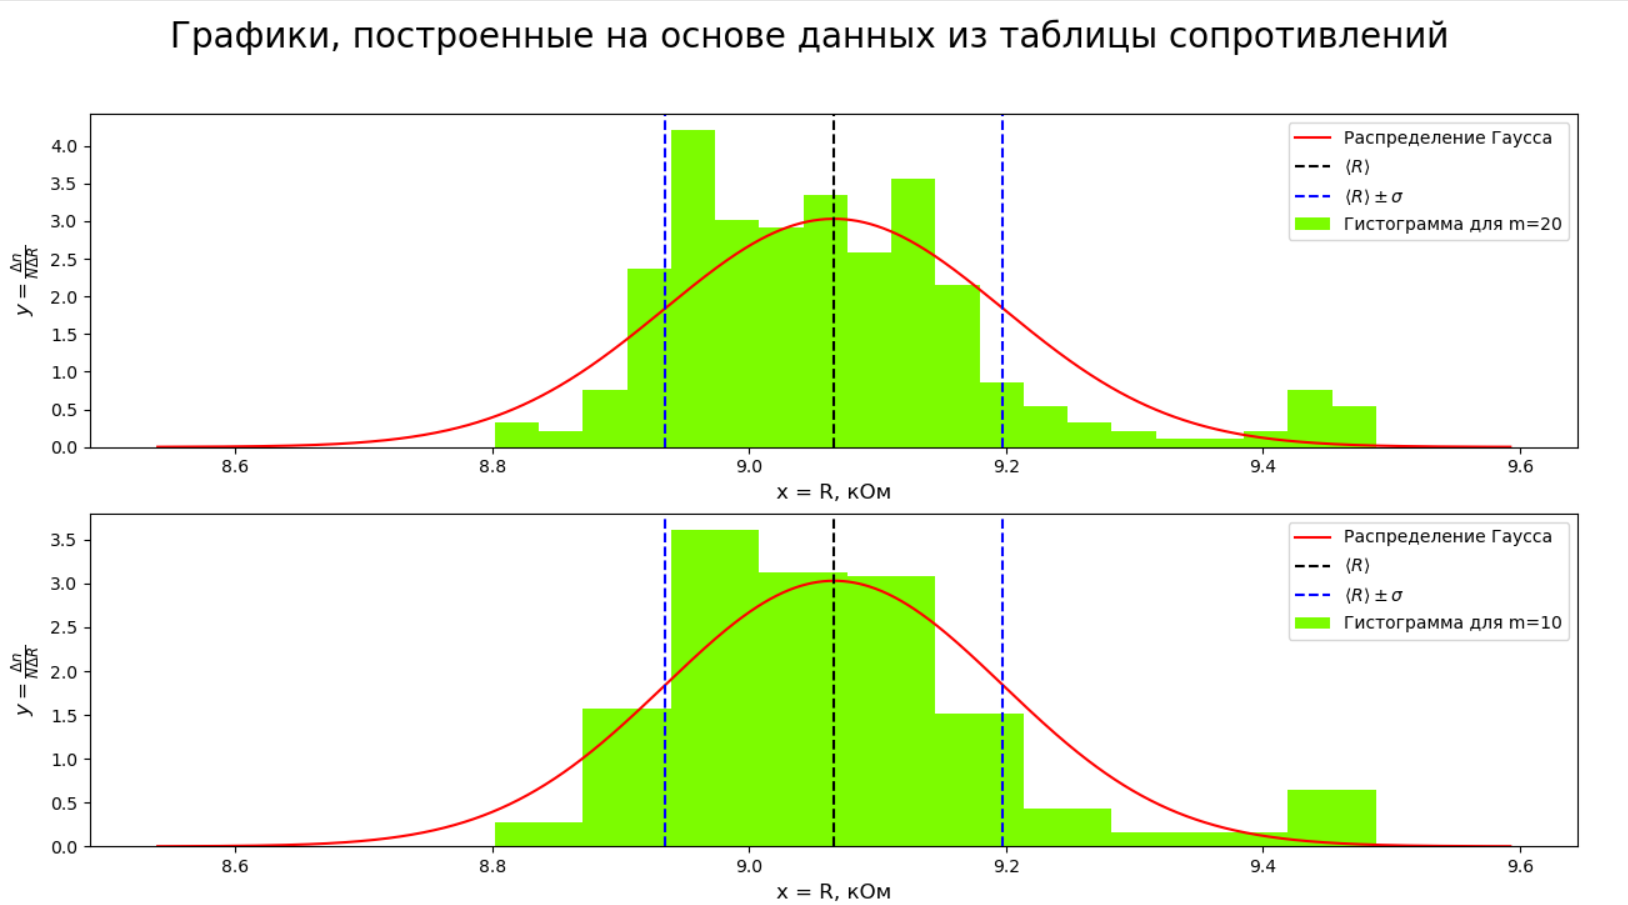
\includegraphics[width=\linewidth]{Graphics-1}
		\end{figure}
	\section*{Вывод:}
		Таким образом, в интервал от $\langle R\rangle - \sigma$ до $\langle R\rangle + \sigma$ укладывается 74$\%$ значений, в интервал от $\langle R\rangle - 2\sigma$ до $\langle R\rangle + 2\sigma$ укладывается 94$\%$ значений, а в интервал от $\langle R\rangle - 3\sigma$ до $\langle R\rangle + 3\sigma$ - 98$\%$. Значит, почти все величины сопротивлений укладываются в 5-процентный интервал $\langle R \rangle \pm 3 \sigma$.
\end{document}
